\documentclass[a4paper,10pt]{article}
\usepackage{polski}
\usepackage[T1]{fontenc}
\usepackage[utf8]{inputenc}
\usepackage{amsfonts}
\usepackage{amsmath}
\usepackage{indentfirst}
\usepackage{graphicx}
\usepackage[scale=0.7]{geometry}
\usepackage[font=small,labelfont=bf]{caption}
\newcommand{\name}{\( \mathbb{O} \)ld-\( \mathbb{S} \)chool \( \mathbb{S} \)hooter }
\title{
	Projekt z programowania obiektowego\\
	Niezbędnik czytelnika}
\author{Daniela Tataruda}

\begin{document}

\maketitle

\section{Wstęp}

Niezbędnik czytelnika jest aplikacją okienkową napisaną w języku Java przy użyciu biblioteki Swing, która umożliwia obsługę interfejsu okienkowego. Aplikacja jest projektem semestralnym z programowania obiektowego na zajęcia w Instytucie Informatyki UWr. Program jest przeznaczony dla osób lubiących czytać i upamiętniać przeczytane przez siebie książki.
\section{Opis programu}
Aplikacja składa się z pięciu okien.
\begin{enumerate}
\item \textbf{Okno główne} - jest to podstawowe okno menu, zawiera logo aplikacji i cztery przyciski, które automatycznie po kliknięciu przenoszą do odpowiednich okien.
\begin{center}
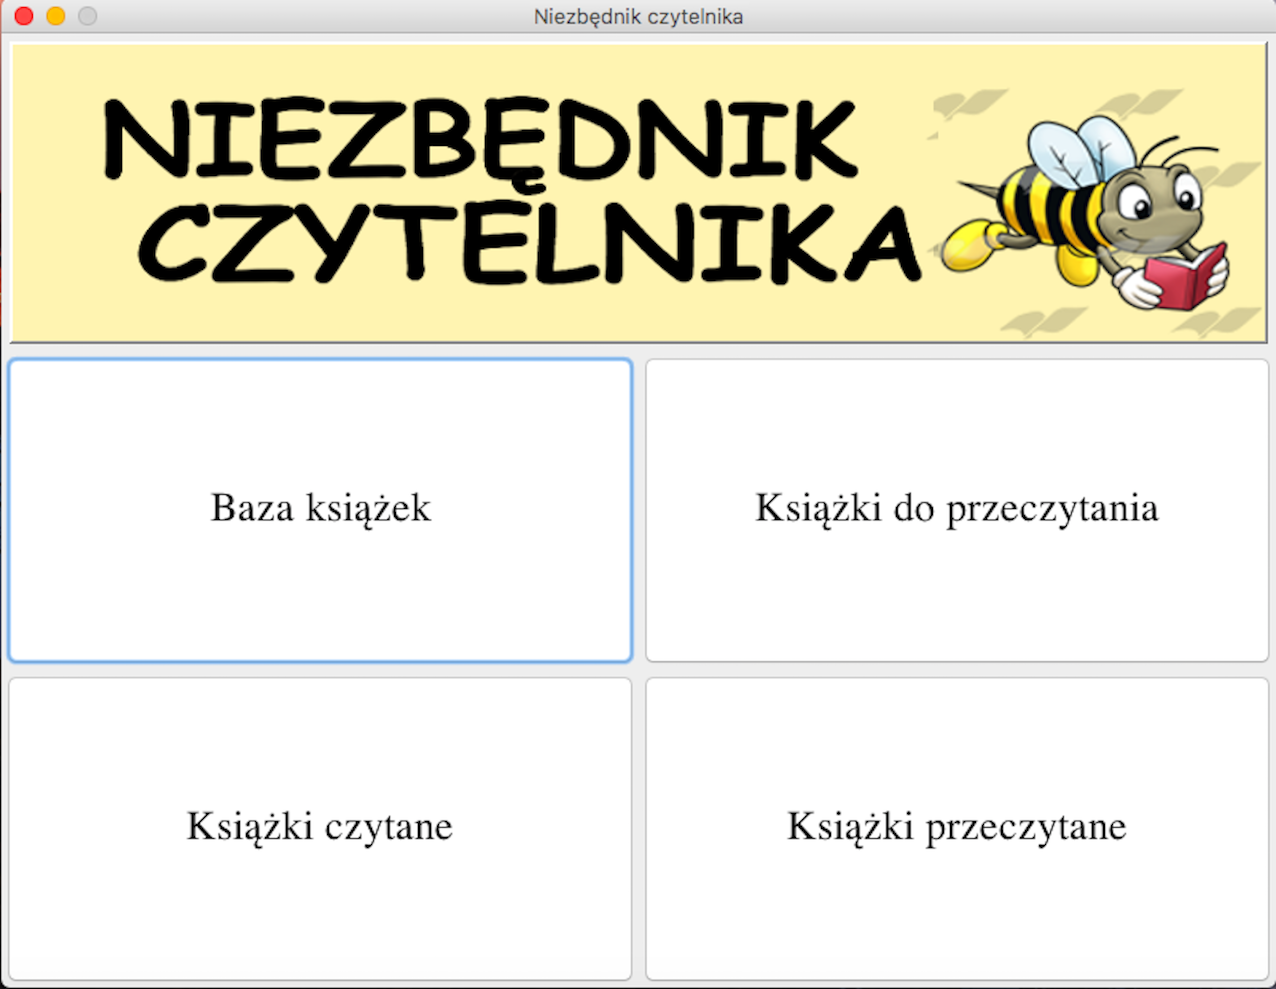
\includegraphics[scale=0.18]{OknoGlowne.png}
\captionof{figure}{ \textit{Okno Główne}.}
\end{center}

\item \textbf{Baza książek} - jest to okno, w którym wyświetlana jest cała podstawowa baza książek. Po prawej stronie wyświetlany jest interfejs zaznaczonej książki i panel z przyciskami pozwalający użytkownikowi wykonać trzy operacje (przeniesienie książki do bazy książek do przeczytania, zaznaczenie, że książka jest w chwili obecnej czytana oraz powrót do okna głównego).
\begin{center}
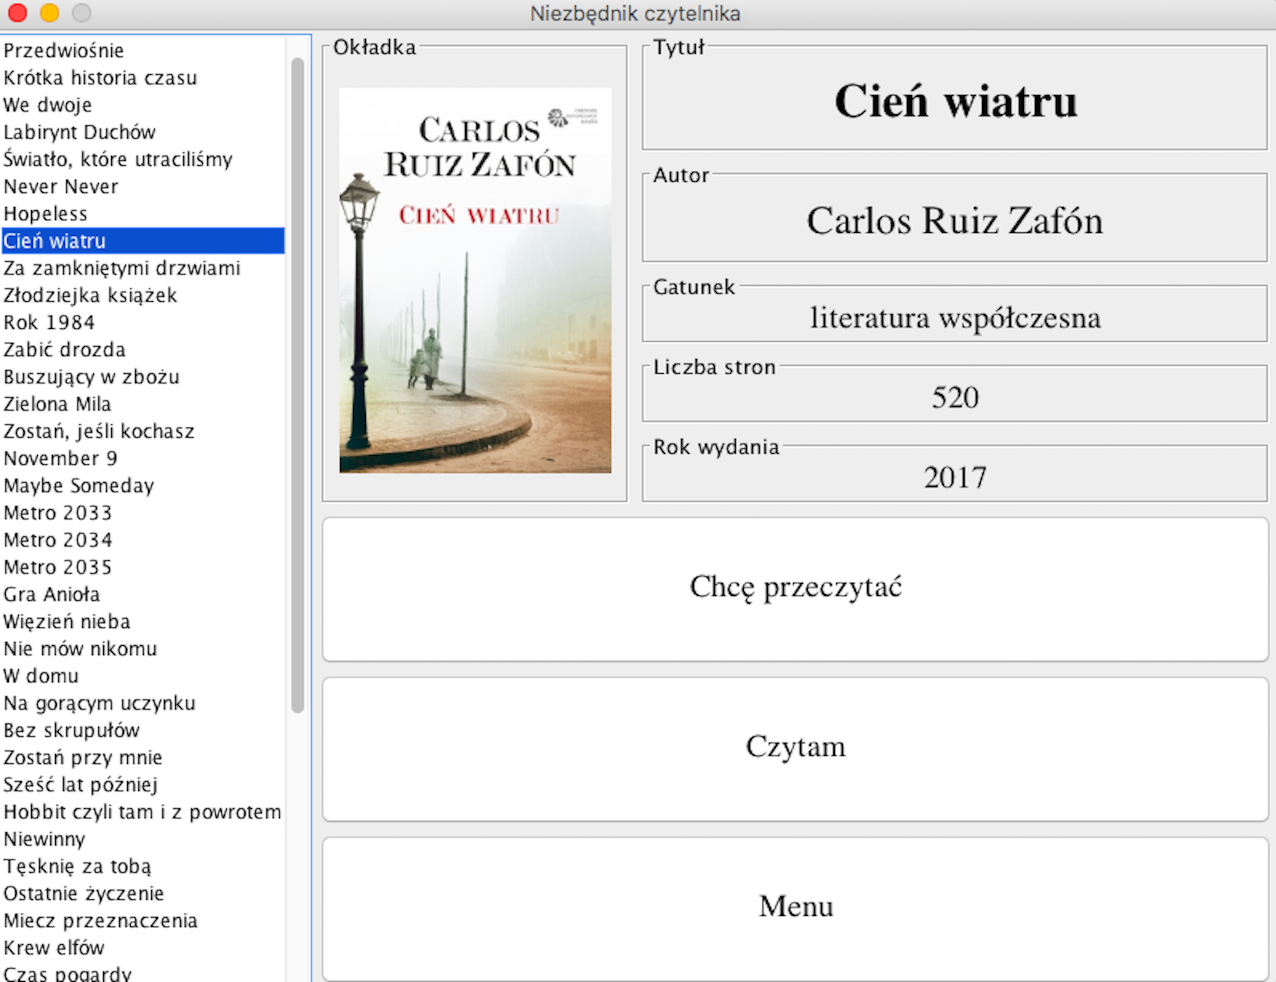
\includegraphics[scale=0.18]{BazaKsiazek.png}
\captionof{figure}{ \textit{Baza książek}.}
\end{center}

\item \textbf{Baza książek do przeczytania} - jest to okno, w którym wyświetlana jest lista książek, które użytkownik zaznaczył jako te, które chce przeczytać. Po prawej stronie (tak jak w poprzednim oknie) wyświetlany jest interfejs zaznaczonej książki i panel z przyciskami pozwalający użytkownikowi wykonać trzy operacje (zaznaczenie, że książka jest w chwili obecnej czytana, ocenienie książki i przeniesienie do bazy książek przeczytanych oraz powrót do okna głównego).
\begin{center}
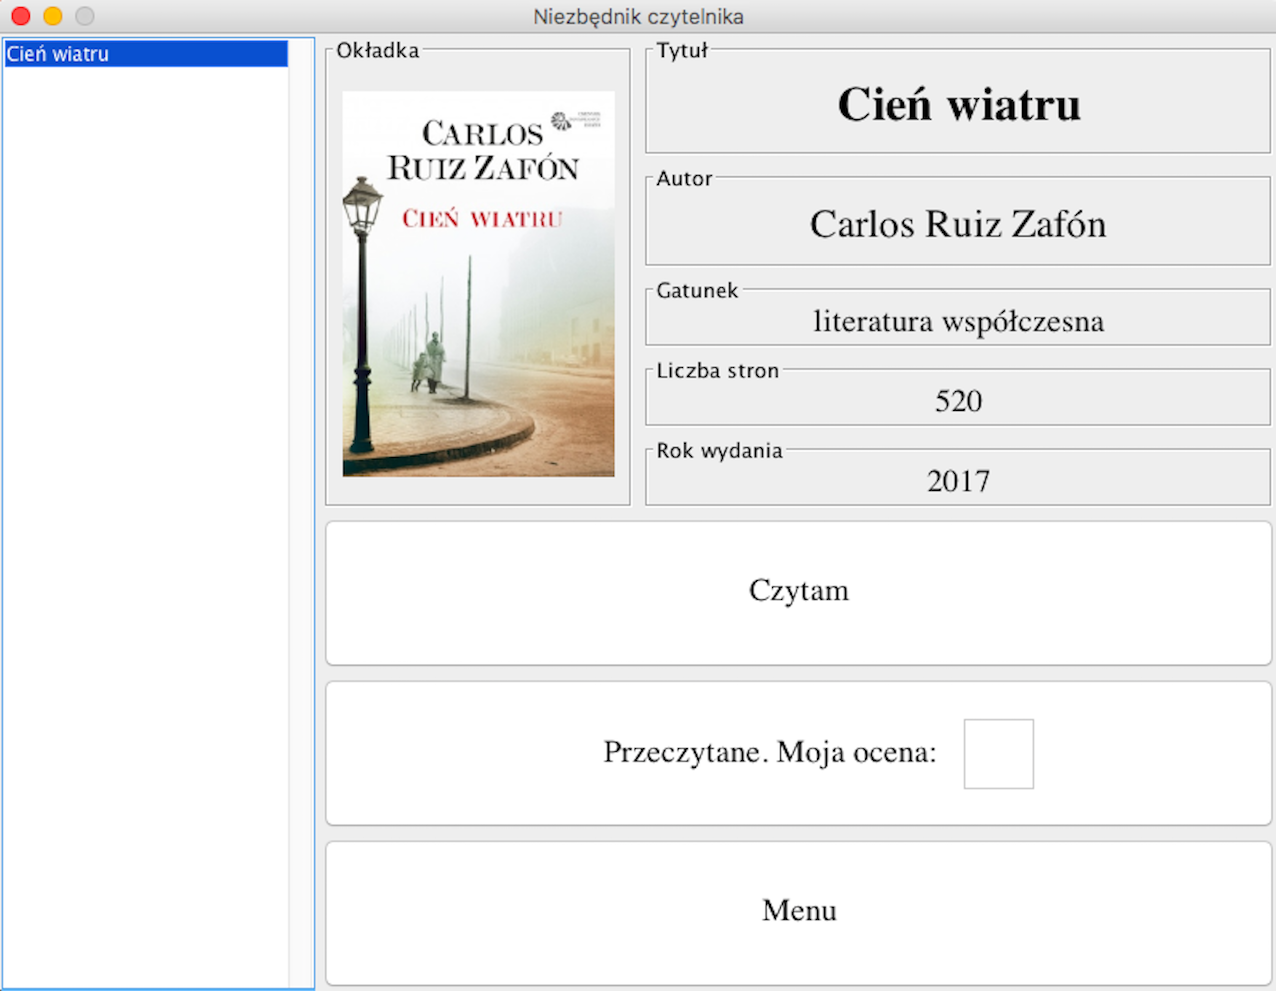
\includegraphics[scale=0.18]{BazaDoPrzeczytania.png}
\captionof{figure}{ \textit{Baza  książek do przeczytania}.}
\end{center}

\item \textbf{Baza książek czytanych } - jest to okno, w którym wyświetlana jest lista książek, które użytkownik zaznaczył jako te, które czyta. Po prawej stronie (tak jak w poprzednich oknach)
wyświetlany jest interfejs zaznaczonej książki i panel z przyciskami pozwalający użytkownikowi wykonać trzy operacje (wprowadzenie liczby przeczytanych stron i zobaczenie jaki postęp w czytaniu został wykonany, ocenienie książki i przeniesienie do bazy książek przeczytanych oraz powrót do okna głównego).
\begin{center}
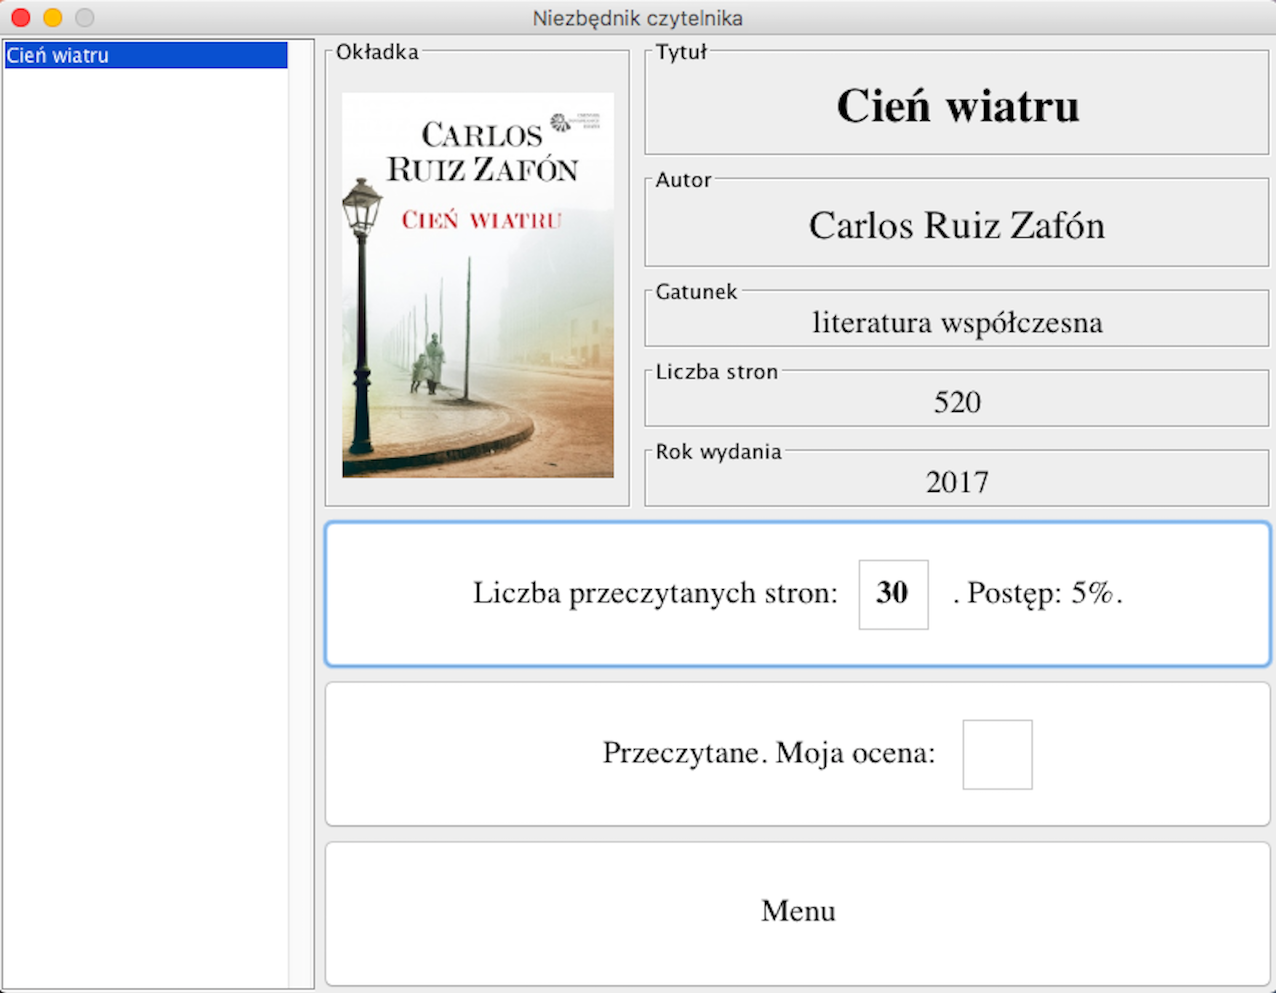
\includegraphics[scale=0.18]{BazaKsiazekCzytanych.png}
\captionof{figure}{ \textit{Baza  książek czytanych}.}
\end{center}

\item \textbf{Baza książek przeczytanych } - jest to okno, w którym wyświetlana jest lista książek, które użytkownik zaznaczył jako te, które przeczytał. Po prawej stronie (tak jak w poprzednich oknach)
wyświetlany jest interfejs zaznaczonej książki i panele z informacjami o ocenie jaką wystawił użytkownik i data przeczytania danej książki. Na dole okna umieszczony jest przycisk, który służy do powrotu do okna głównego aplikacji.
\begin{center}
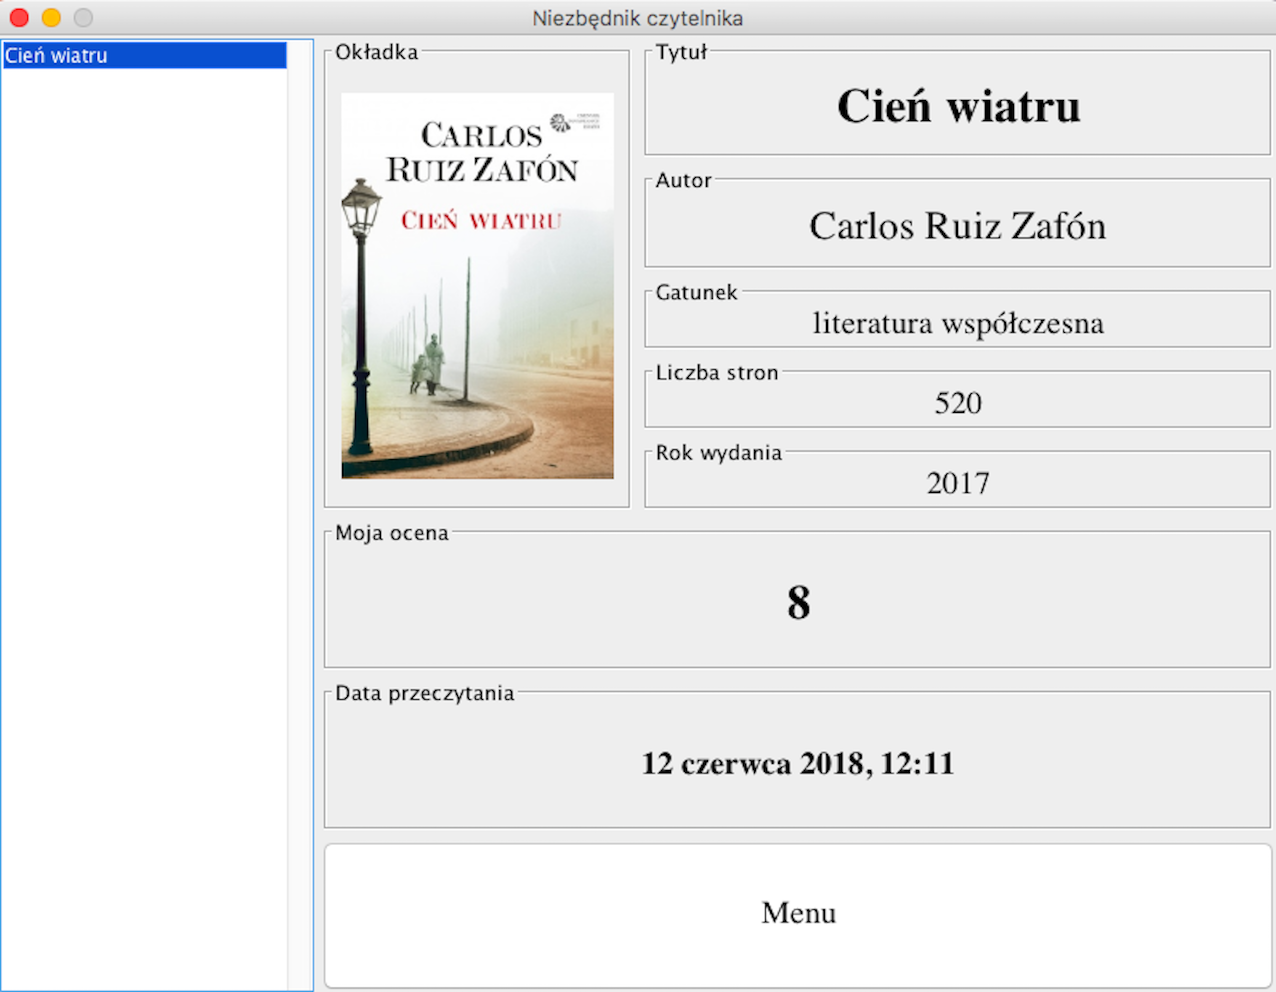
\includegraphics[scale=0.18]{BazaPrzeczytane.png}
\captionof{figure}{ \textit{Baza  książek przeczytanych}.}
\end{center}
\section{Analiza obiektowa}
\subsection{Lista klas z opisem}
\subsubsection{Projekt}
Klasa z jedną statyczną metodą main(), która uruchamia program.
\begin{center}
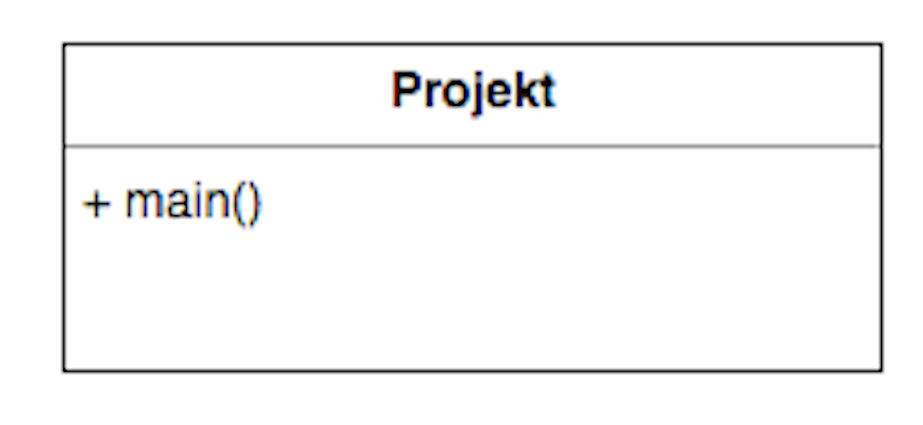
\includegraphics[scale=0.18]{UML8.png}
\captionof{figure}{ \textit{Schemat klasy Projekt}.}
\end{center}

\subsubsection{Okno}
Klasa dziedzicząca po \textit{JFrame}. Ustawia domyślne wartości dla okna (resizable(false), wymiary, wyjście).

\subsubsection{OknoGlowne}
Klasa dziedzicząca po \textit{Okno}. Kontroluje i ustawia wszystkie przyciski oraz obrazki pojawiające się w pierwszym podstawowym oknie aplikacji.

\subsubsection{OknoKsiazki}
Klasa dziedzicząca po \textit{Okno}. Zawiera panel przesuwany z listą książek z bazy podanej jako parametr w konstruktorze oraz panel książki z klasy \textit{PanelKsiazki}.

\begin{center}
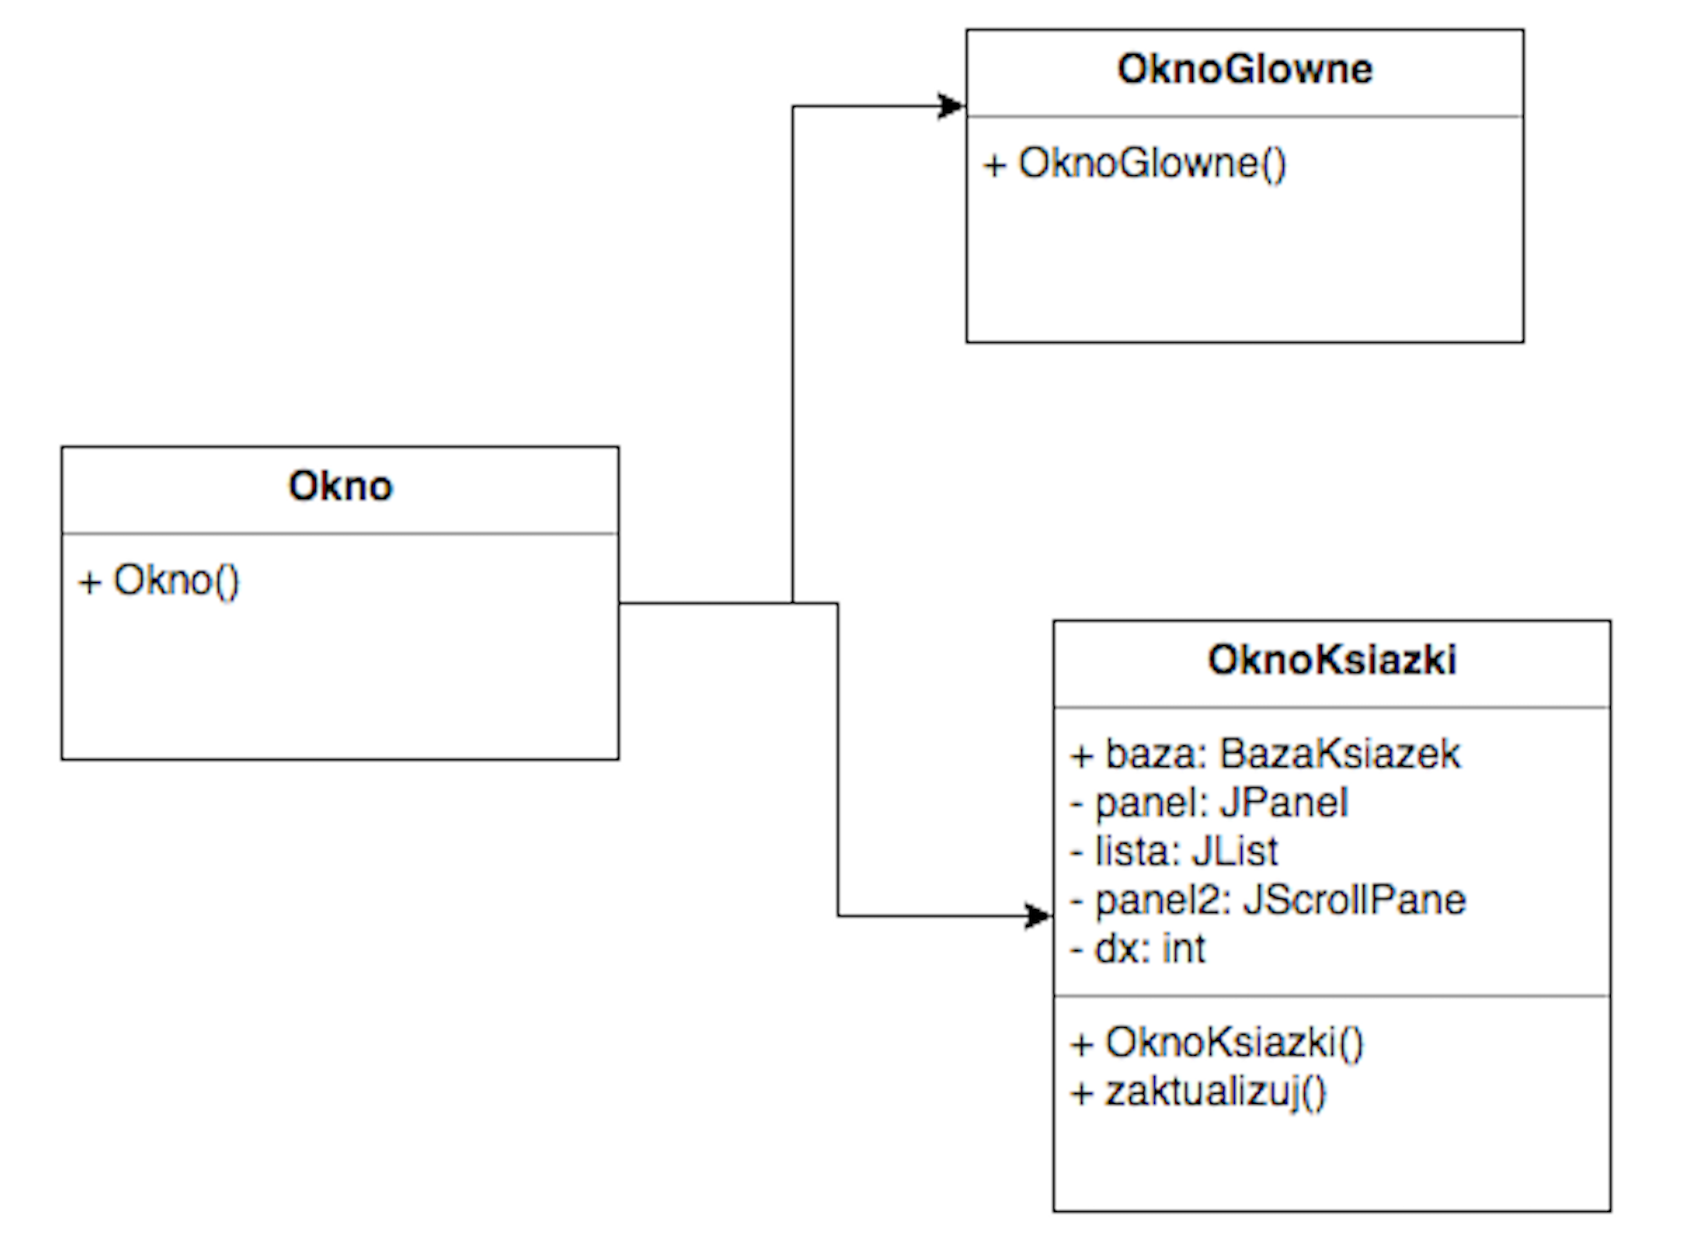
\includegraphics[scale=0.18]{UML3.png}
\captionof{figure}{ \textit{Schemat klas dziedziczących po \textbf{Okno}}.}
\end{center}

\subsubsection{Panel}
Klasa dziedzicząca po \textit{JPanel}. Ma w sobie metodę \textit{dodajKomponent} pozwalającą dodawać obiekty w podanych miejscach i z odpowiednimi parametrami podanymi jako argumenty funkcji.

\subsubsection{PanelKsiazki}
Klasa dziedzicząca po \textit{Panel}. Jest to klasa ustawiająca cały interfejs książki znajdujący się w oknie książki, korzystająca z funkcji \textit{dodajKomponent} i posiadająca metodę \textit{dodajPrzyciskiSpecjalne} oraz ustawiająca przyciski do poruszania się po oknach.

\begin{center}
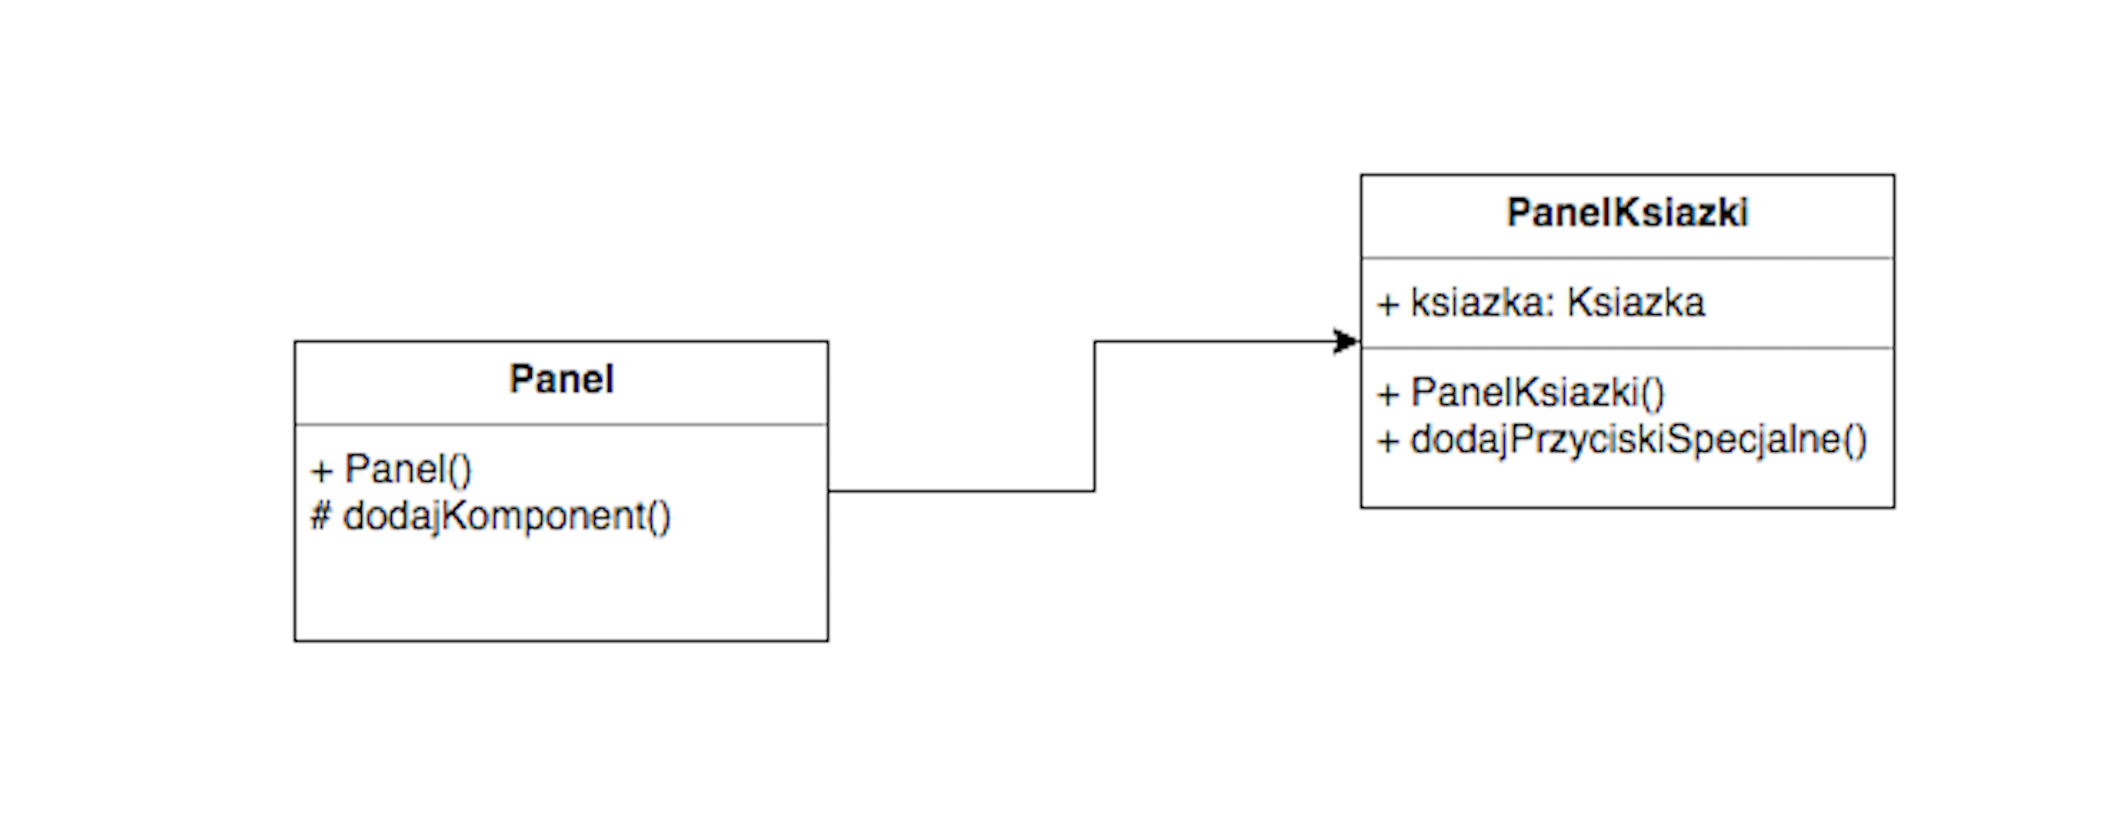
\includegraphics[scale=0.18]{UML4.png}
\captionof{figure}{ \textit{Schemat klas dziedziczących po \textbf{Panel}}.}
\end{center}

\subsubsection{Ksiazka}
Klasa definiująca obiekt książki, czyli bazowy obiekt programu. Ma w sobie pola określające daną książkę oraz metody wydobywania tych pól, ponieważ są to pola chronione (niedostępne z zewnątrz klasy). Zaimplementowana jest tutaj także metoda pobierająca okładkę z folderu \textit{grafiki}.

\subsubsection{KsiazkaDoPrzeczytania}
Klasa dziedzicząca po \textit{Ksiazka} definiująca obiekt książki do przeczytania.

\subsubsection{KsiazkaCzytana} 
Klasa dziedzicząca po \textit{Ksiazka} definiująca obiekt książki czytanej. Posiada ona dodatkowe pole trzymające liczbę stron aktualnie przeczytanych i metodę obliczającą postęp w czytaniu.

\subsubsection{KsiazkaPrzeczytana}
Klasa dziedzicząca po \textit{Ksiazka} definiująca obiekt książki przeczytanej. Posiada ona dodatkowe pola oceny i daty oraz metodę pobierającą i wypisująca datę.

\begin{center}
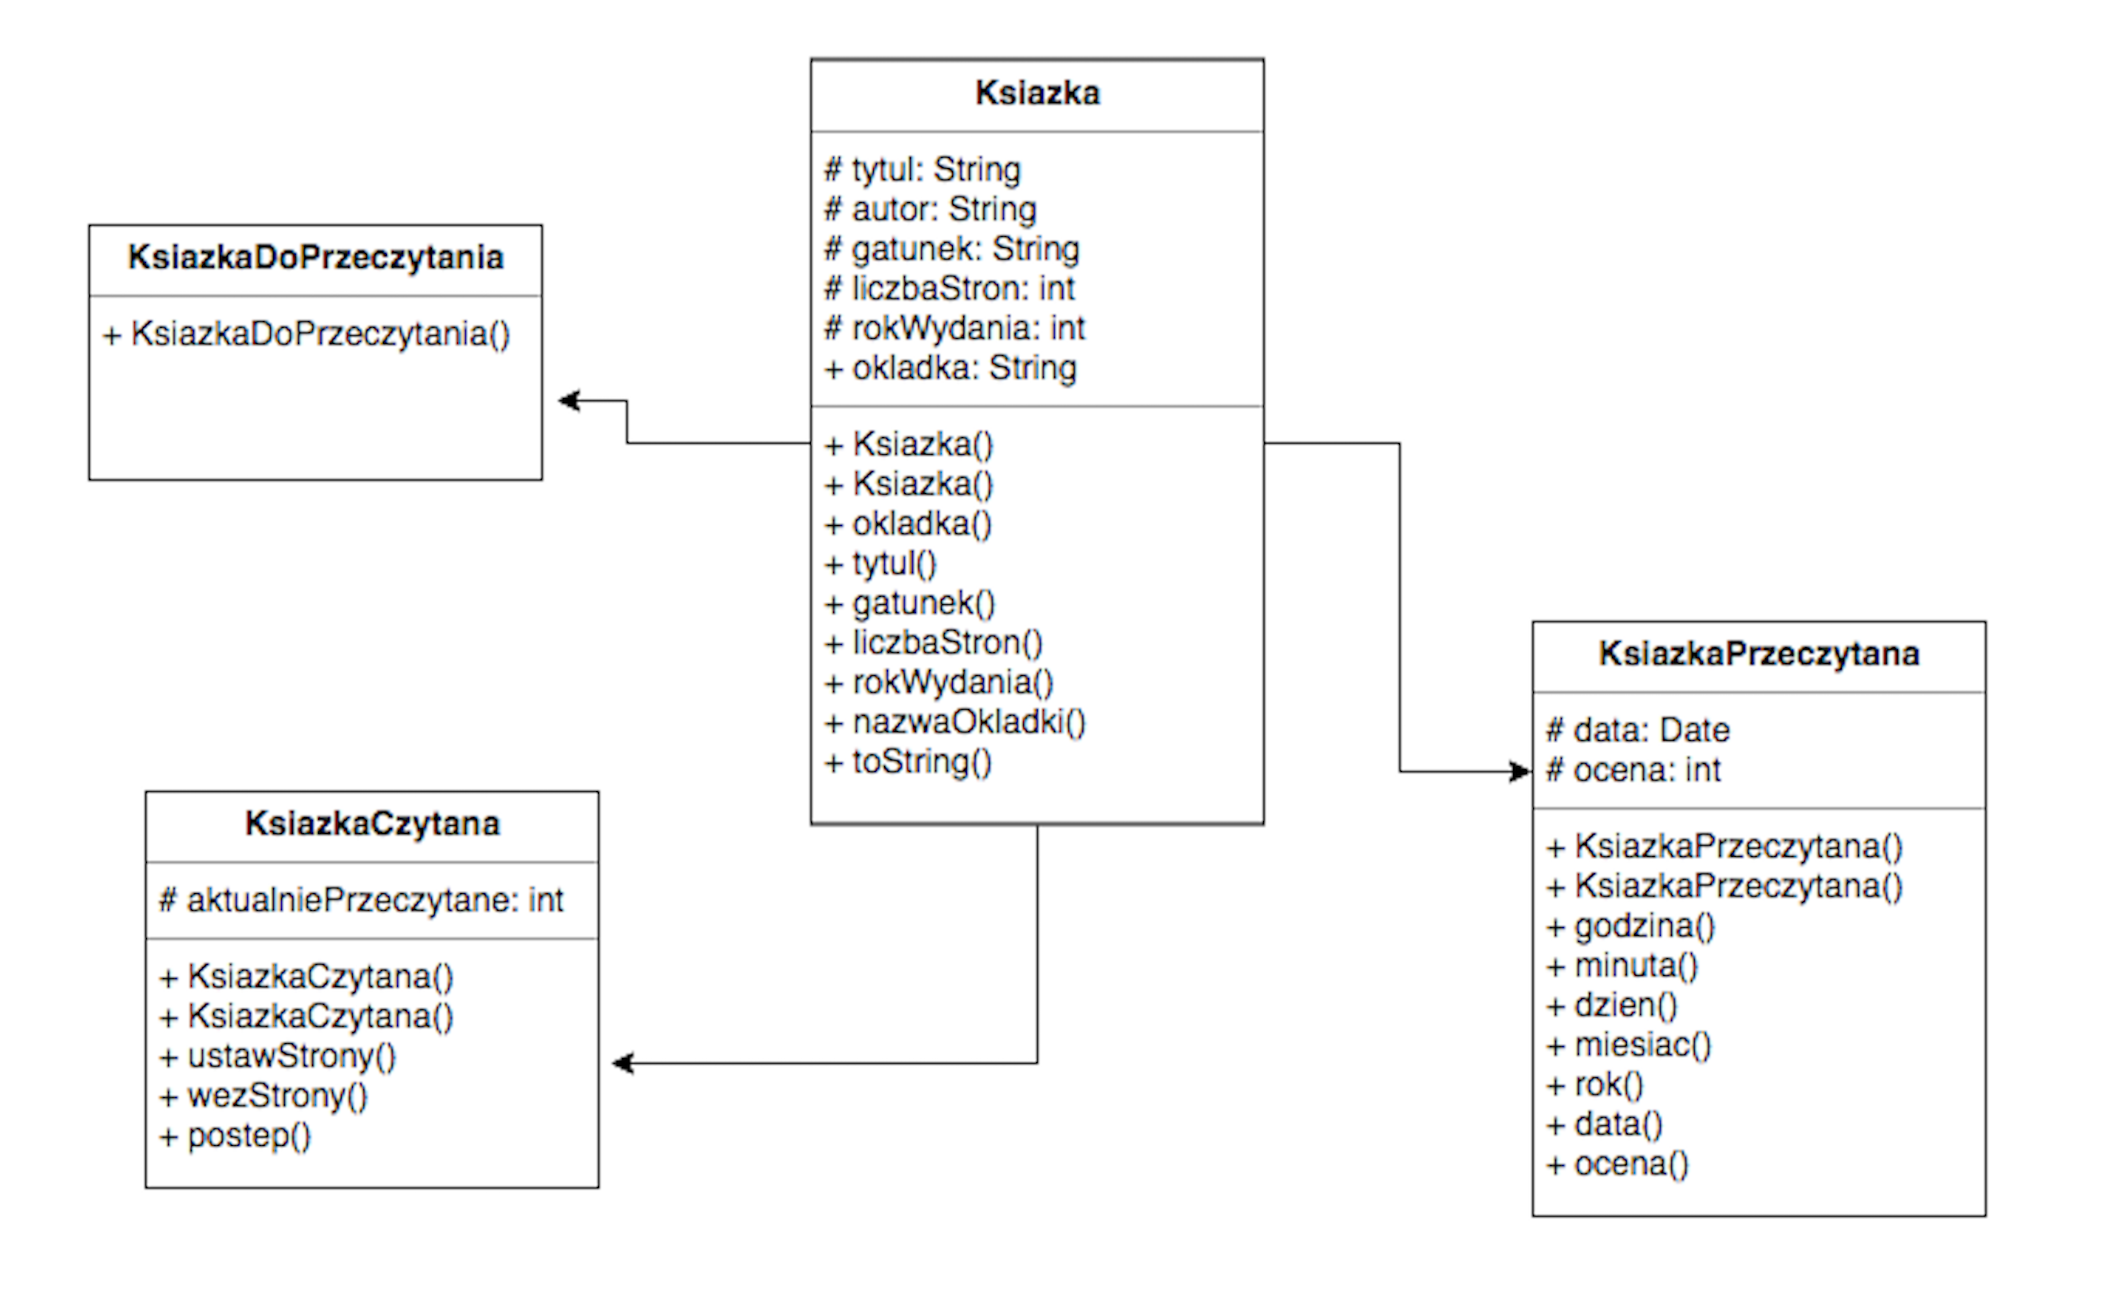
\includegraphics[scale=0.18]{UML1.png}
\captionof{figure}{ \textit{Schemat klas dziedziczących po \textbf{Ksiazka}}.}
\end{center}

\subsubsection{BazaKsiazek}
Klasa trzymająca, czytająca i zapisująca bazę książek w postaci pliku z rozszerzeniem .bin. Implementuje interfejs \textit{Serializable}. Baza jest przechowywana w postaci listy obiektów klasy \textit{Ksiazka}. Ma standardowe metody dodawania i usuwania elementów z listy oraz dwie metody obsługujące zapisywanie i czytanie z plików binarnych.

\subsubsection{BazaDoPrzeczytania}
Klasa dziedzicząca po \textit{BazaKsiazek} trzymająca bazę książek do przeczytania.

\subsubsection{BazaCzytane}
Klasa dziedzicząca po \textit{BazaKsiazek} trzymająca bazę książek czytanych.

\subsubsection{BazaPrzeczytane}
Klasa dziedzicząca po \textit{BazaKsiazek} trzymająca bazę książek przeczytanych.

\begin{center}
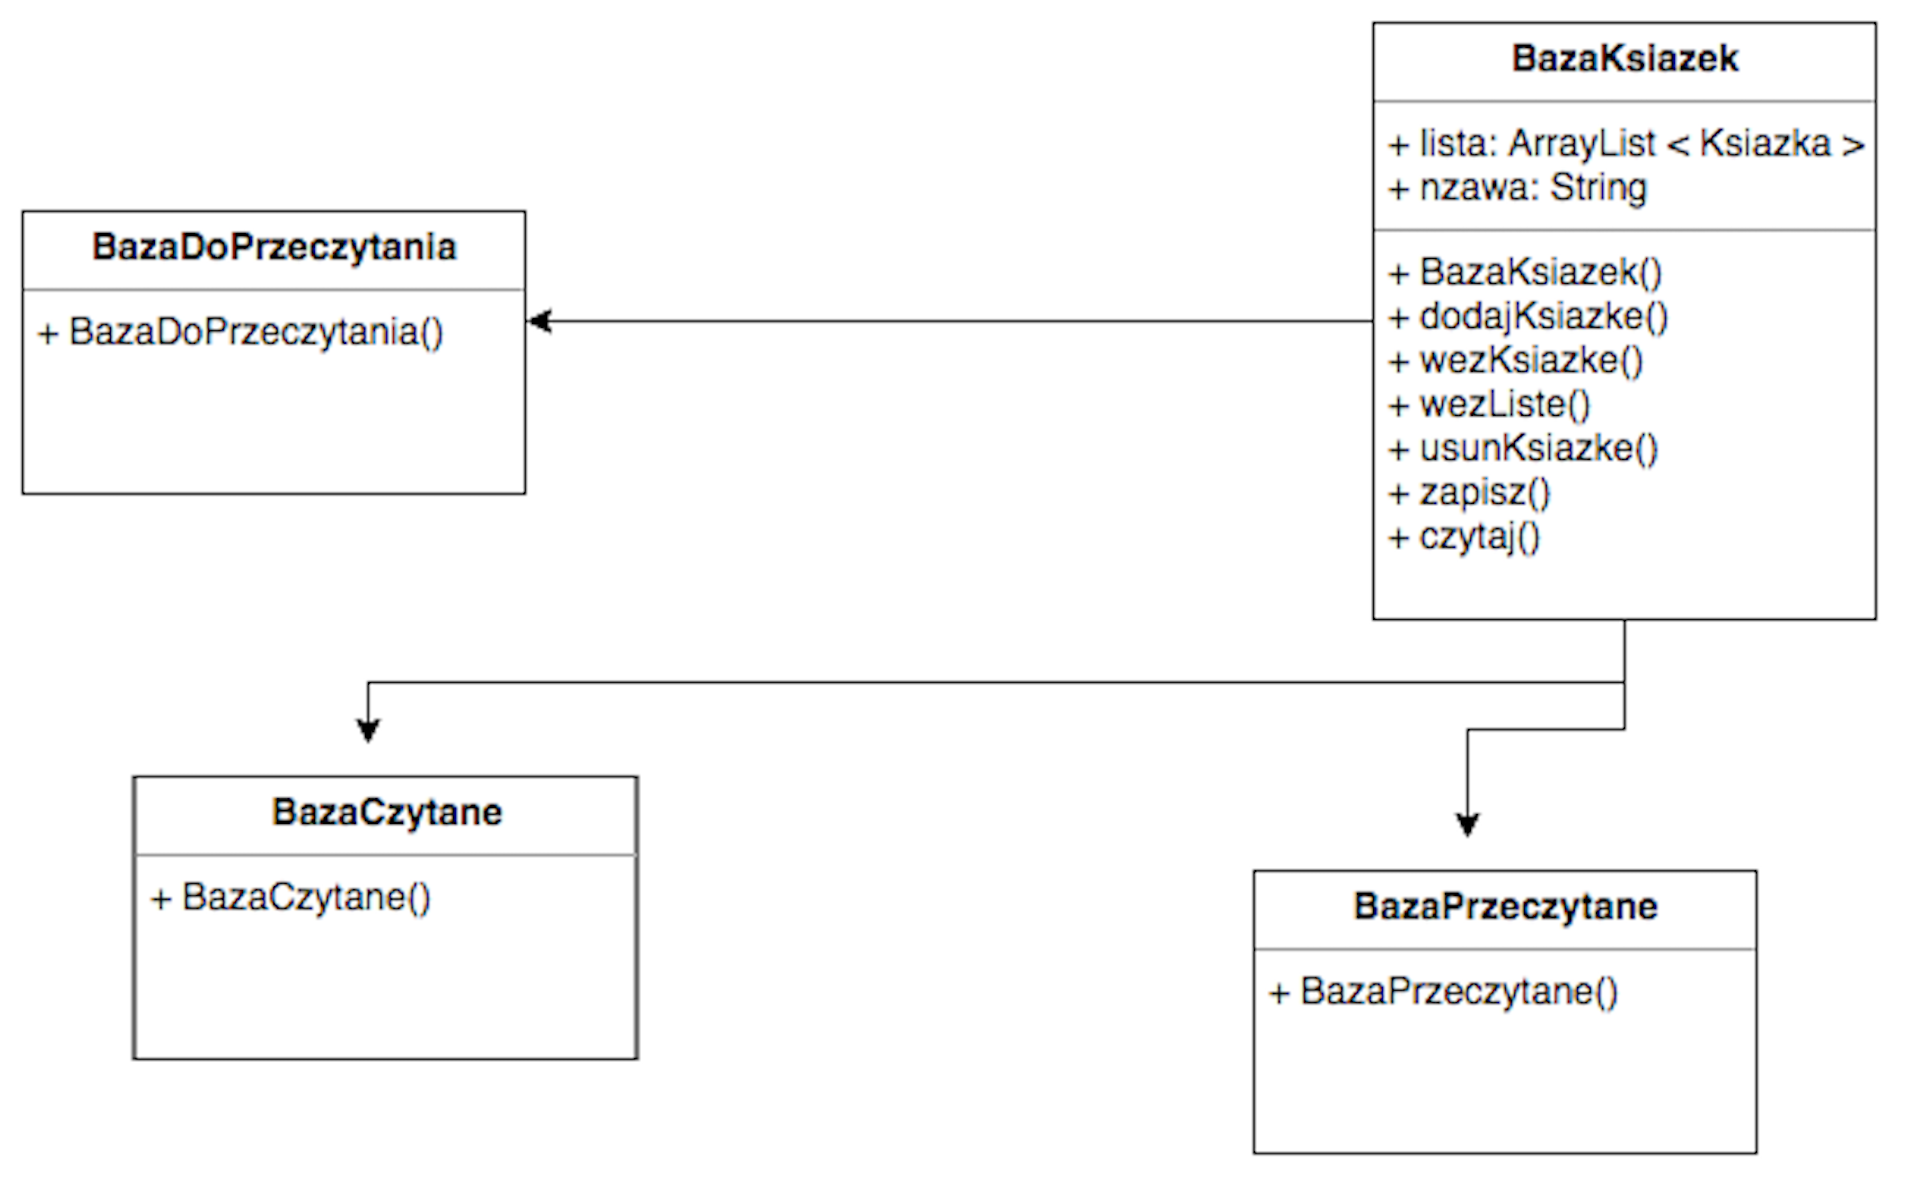
\includegraphics[scale=0.18]{UML2.png}
\captionof{figure}{ \textit{Schemat klas dziedziczących po \textbf{BazaKsiazek}}.}
\end{center}

\subsubsection{MojPrzycisk}
Klasa dziedzicząca po \textit{JButton}. Pomocnicza klasa definiująca przycisk, jego działanie i rozmieszczenie w oknie w zależności od parametrów w konstruktorze.

\subsubsection{PrzyciskChcePrzeczytac}
Klasa dziedzicząca po \textit{JButton}. Tworzy przycisk dodawania książki do bazy książek do przeczytania.

\subsubsection{PrzyciskCzytam}
Klasa dziedzicząca po \textit{JButton}. Tworzy przycisk dodawania książki do bazy książek czytanych.

\begin{center}
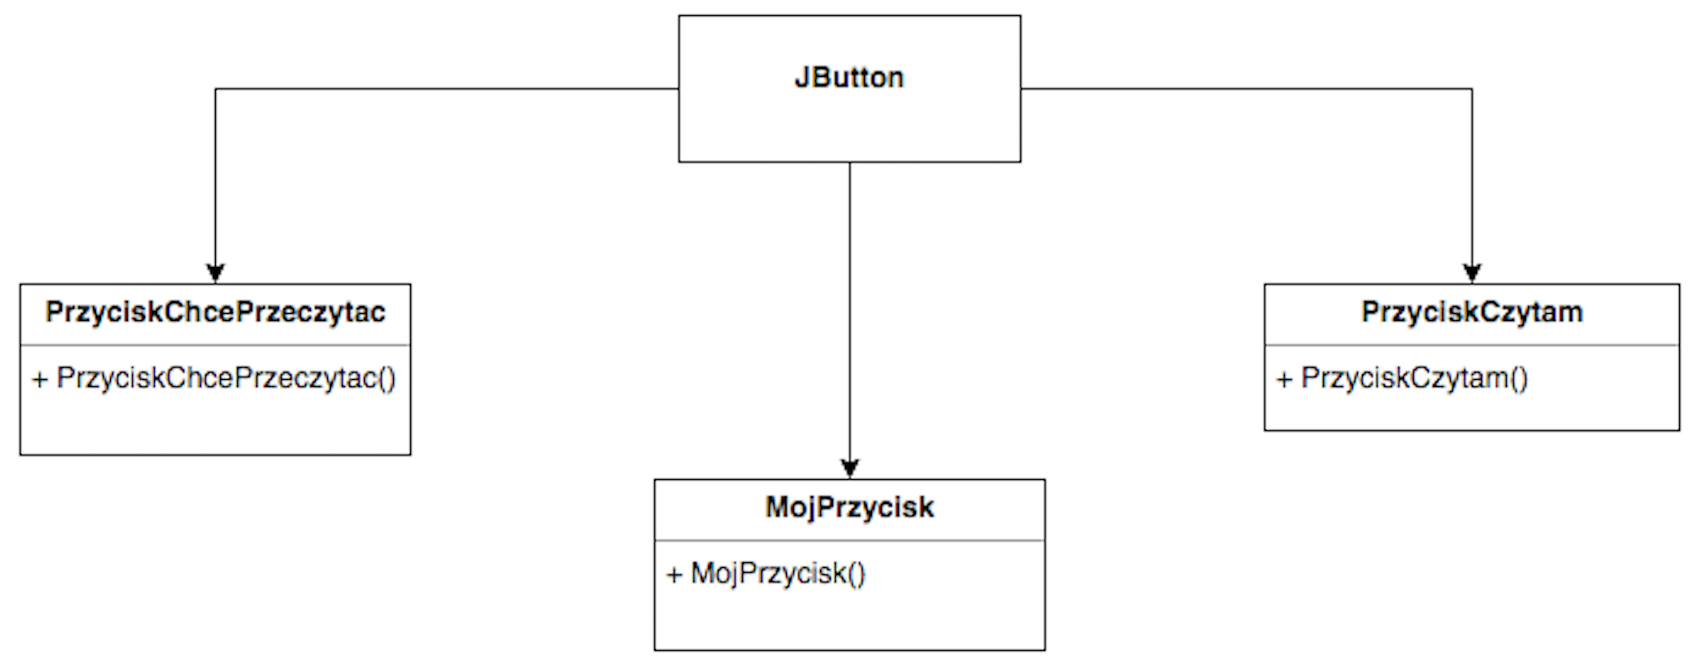
\includegraphics[scale=0.18]{UML7.png}
\captionof{figure}{ \textit{Schemat klas dziedziczących po \textbf{JButton}}.}
\end{center}

\subsubsection{PrzyciskPostep}
Klasa dziedzicząca po \textit{JPanel}. Tworzy przycisk który po podaniu liczby stron aktualnie przeczytanych i kliknięciu podaje nam nasz obecny postęp czytania danej książki.

\subsubsection{PrzyciskPrzeczytane}
Klasa dziedzicząca po \textit{JButton}. Tworzy przycisk dodawania książki do bazy książek przeczytanych z możliwością ocenienia książki.

\begin{center}
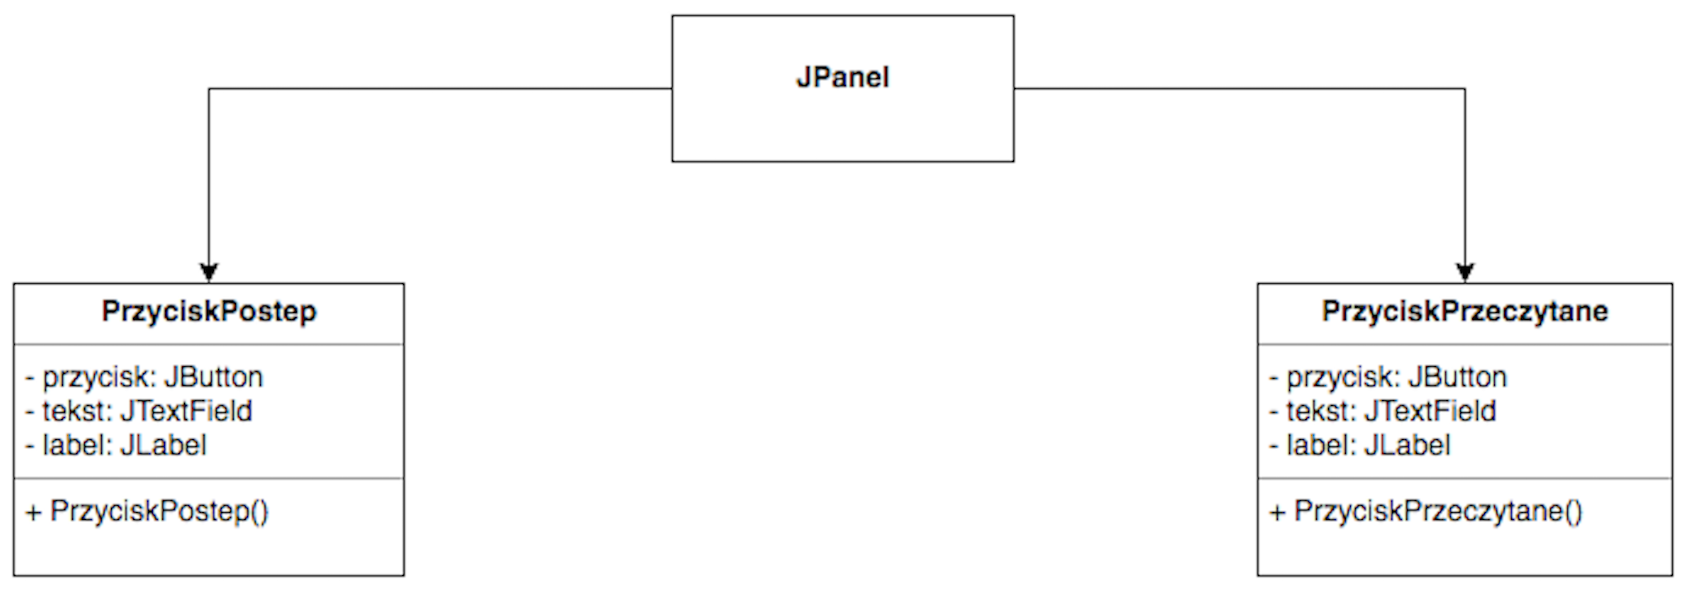
\includegraphics[scale=0.18]{UML5.png}
\captionof{figure}{ \textit{Schemat klas dziedziczących po \textbf{JPanel}}.}
\end{center}

\subsubsection{MojLabel}
Klasa dziedzicząca po \textit{JLabel} definiująca wszystkie pola tekstowe i obrazkowe w aplikacji.

\begin{center}
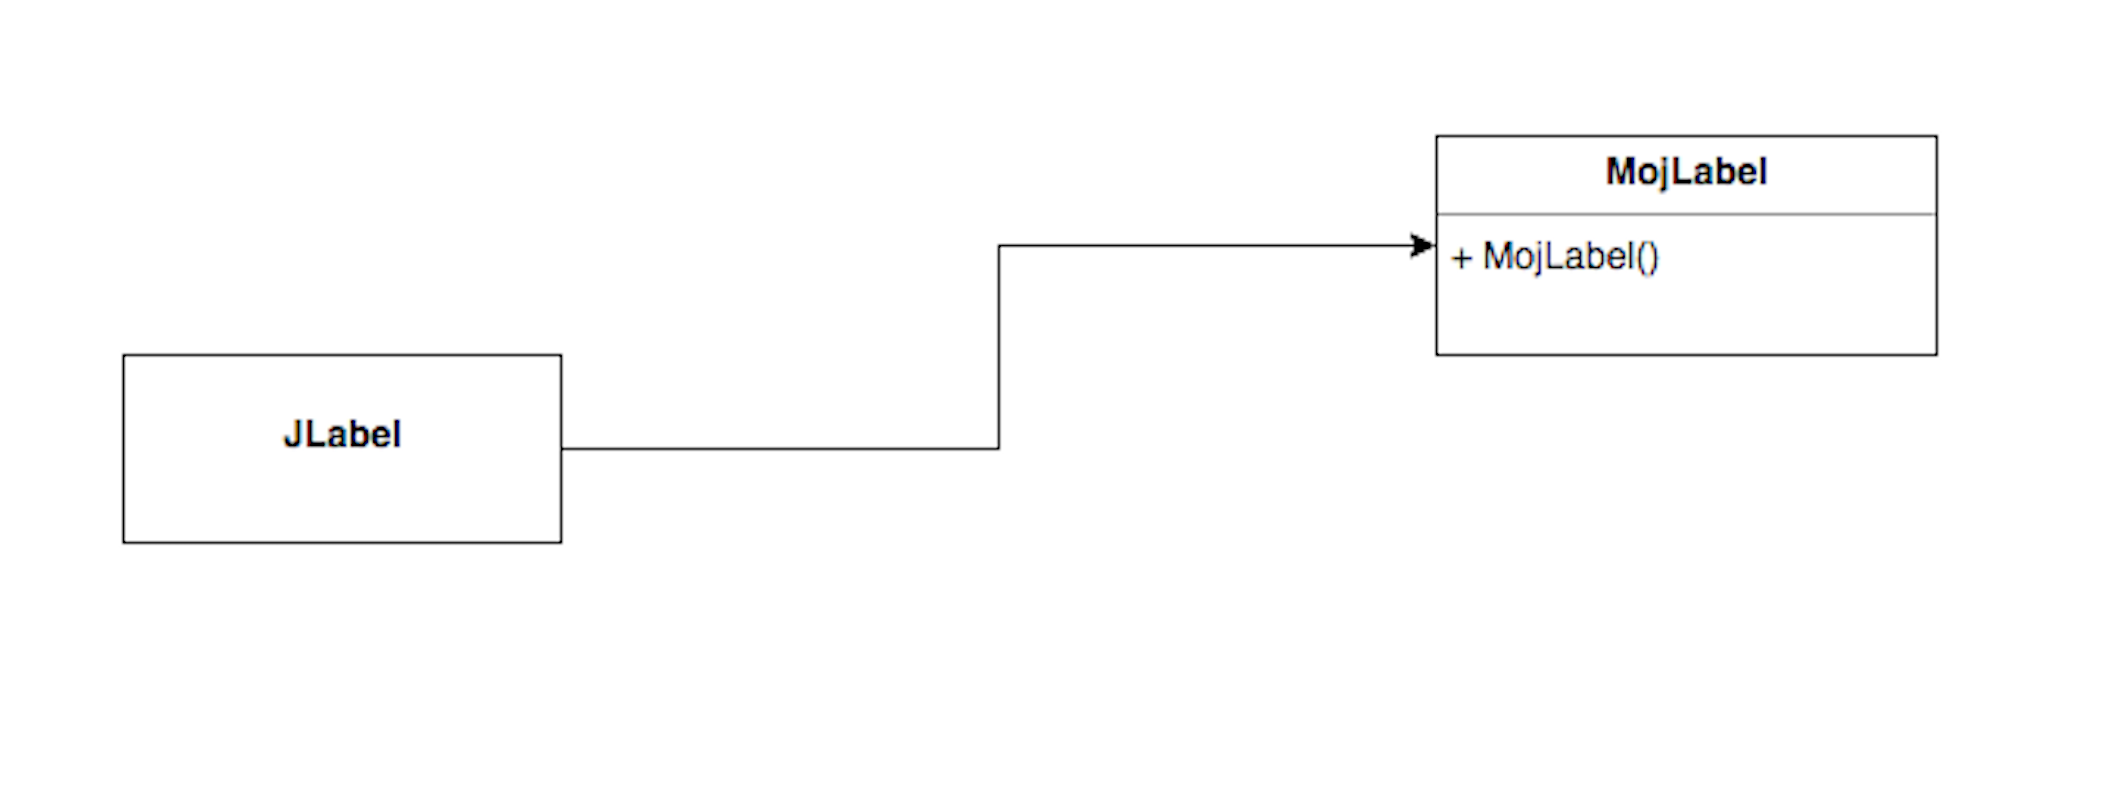
\includegraphics[scale=0.18]{UML6.png}
\captionof{figure}{ \textit{Schemat klas dziedziczących po \textbf{JLabel}}.}
\end{center}

\subsection{Realizowana funkcjonalność}
\subsubsection{Użytkownik}
Każdy użytkownik ma równy dostęp do aplikacji. W aplikacji nie zostały umieszczone żadne ukryte możliwości, więc użytkownik może korzystać z wszystkich funkcji podanych w opisie programu.
\subsubsection{Programista}
Aplikacja jest przystosowana do dalszego rozwoju. Więcej o tym w rozdziale \textbf{Dalsza rozbudowa}. Poza rozszerzeniem kodu programista może dowolnie dodawać książki do bazy.
\section{Dalsza rozbudowa}
Aplikacja była pisana w dość krótkim czasie, istnieje zatem wiele możliwości rozwoju. Jedną z ważniejszych rzeczy do rozbudowy jest panel umożliwiający użytkownikowi dodanie własnej książki do bazy w przypadku gdy dana książka jeszcze w niej nie istnieje. Możliwe jest także wprowadzenie różnego rodzaju filtrowania bazy książek (po gatunku, autorze, roku wydania).

\end{enumerate}






\end{document}